\documentclass[11pt,letterpaper,final]{report}
\usepackage[utf8]{inputenc}
\usepackage[english]{babel}
\usepackage{amsmath}
\usepackage{indentfirst}
\usepackage{amsfonts}
\addto{\captionsenglish}{\renewcommand{\bibname}{\LARGE{References}}}
\usepackage{pdfpages}
\usepackage{subcaption}
\usepackage{etoolbox}
\usepackage{amssymb}
\usepackage[font=small,labelfont=bf]{caption}
\usepackage{hanging}
\usepackage{notoccite}
\usepackage{float}
\usepackage{makeidx}
\usepackage{color}
\usepackage{titlesec}
\usepackage{gensymb}
\usepackage{hyperref}
\usepackage{graphicx}
\usepackage{lmodern}

\makeatletter
% section from book
%\newcommand\section{\@startsection {section}{1}{\z@}%
%                                   {-3.5ex \@plus -1ex \@minus -.2ex}%
%                                   {2.3ex \@plus.2ex}%
%                                   {\normalfont\Large\bfseries}}
\renewcommand\chapter{\@startsection {chapter}{0}{\z@}%
                                   {-4.5ex \@plus -1ex \@minus -.2ex}%
                                   {3.3ex \@plus.2ex}% 
                                   {\normalfont\LARGE\textbf}}


\makeatletter



\setlength{\parskip}{\baselineskip}%
\setlength{\parindent}{0pt}%






\usepackage{fourier}
\usepackage[left=1in,right=1in,top=1in,bottom=1in]{geometry}

\titleformat{\chapter}{\normalfont\huge}{\thechapter.}{20pt}{\huge\bf}
\titlespacing*{\chapter}{0pt}{-.5in}{20pt}
\author{Charles Hammond \\ Jaime Luo \\ Jacob Newman}


\begin{document}



\begin{center}

\begin{huge} 

\begin{Huge}\textbf{Work Plan} \end{Huge} \\~\\  UV System Replacement/UVT Requirement Reduction \\~\\
\end{huge}


\begin{Large} \textit{pHlux Engineering} \end{Large}



\begin{large}

\vspace{100pt}
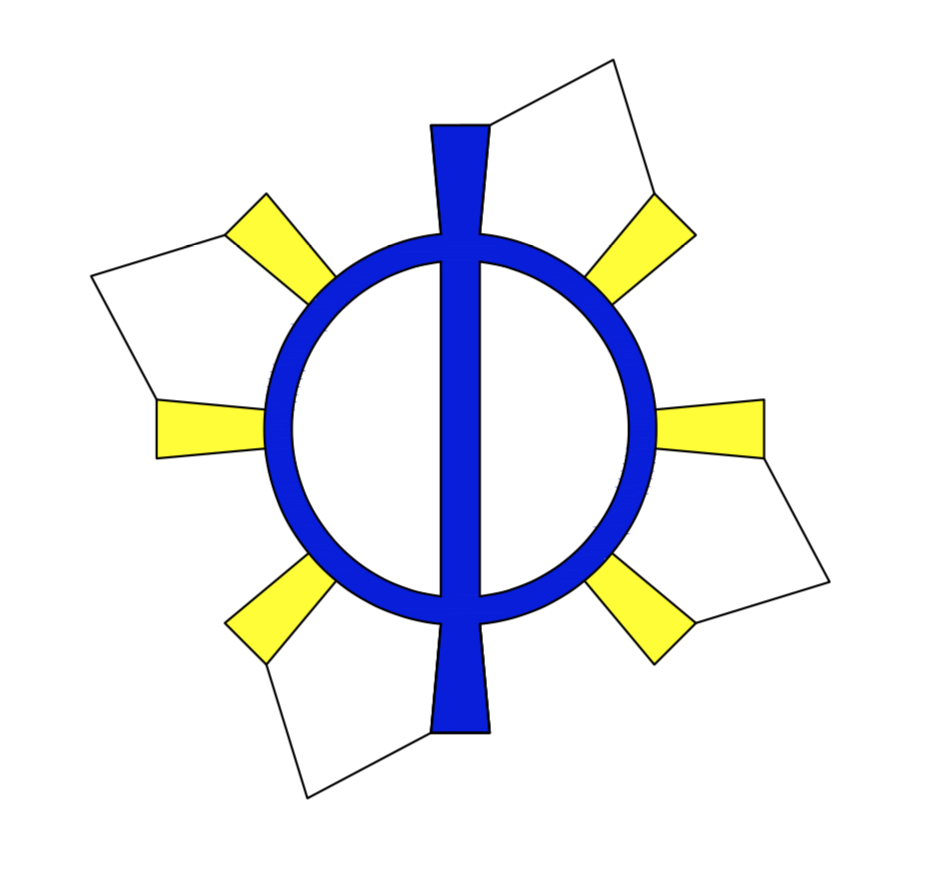
\includegraphics[height=1.5in]{wp1}\\
\end{large}

\vspace{100pt}


\begin{tabular}{ll}
    \textbf{Prepared by:}&Charles Hammond\\
                         & Jaime Luo\\
                         & Jacob Newman\\
                         & \\~\\
    \textbf{Prepared for:}& Colleen Bronner\\
                         & \\~\\
    \textbf{Finalized on:}& \today\\ 

\end{tabular}

\end{center}

\pagenumbering{gobble}


\newpage
\setcounter{page}{0}

\chapter*{Executive Summary}
\pagenumbering{roman} 

    \addcontentsline{toc}{chapter}{Executive Summary}

    This report contains the storm water management design requested by the city of Davis, California, on April 18th, 2018. The sources of stormwater are a tarmac, a grass-covered park, and a housing developement. The design includes a conveyance channel, gutters, inlets and a storm sewer for the housing development, a culvert, and a detention pond. The design is based on a 10-year storm \cite{UCDNews},  \cite{TrojanUV1},  \cite{TrojanLowUVT}, \cite{NPDES}



    
    
\newpage
\setlength{\parskip}{0pt}%
\tableofcontents
\newpage
\listoffigures

\setlength{\parskip}{\baselineskip}%
\addcontentsline{toc}{chapter}{List of Figures}


\newpage
\chapter*{Nomenclature}
\addcontentsline{toc}{chapter}{Nomenclature}

\begin{table}[htbp]
\centering
\begin{tabular}{ccc}
\textbf{Symbol/Initialism} & \textbf{Meaning} & \textbf{Units} \\
\hline
NPDES & National Pollution Discharge Elimination System &  \\
UVT & Ultraviolet Transmissivity & \\
WWTP & Wastewater Treatment Plant & \\
CVRWQCB & Central Valley Regional Water Quality Control Board & \\
MPN & Most probable number &  \\
mgd & Million gallons per day & $10^6$ gal/day \\






\end{tabular} 
\end{table}


\newpage
\setcounter{chapter}{0}
\setcounter{figure}{0}
\setcounter{section}{0}



\chapter{Statement of Problem}
\setcounter{page}{0}
\pagenumbering{arabic}
There are two problems that this project aims to solve for the UC Davis wastewater treatment plant (WWTP). First, the minimum UVT requirement of 55\% in the NPDES permit governing the plant results in yearly violations and fines, even though the tertiary effluent can meet bacterial requirements when UVT drops below 55\%. These violations are undesirable both financially, as the fines add up year after year, and legally, because willfully violating the law is not a viable or responsible solution. To resolve this, the UCD Utilities Division has requested a letter to the Water Board that justifies, based on data and rigorous testing, the reduction or removal of the UVT limit.

Second, the UV disinfection system is nearing the end of its planned service life and is in need of replacement. Because the WWTP discharges to Putah Creek, the Arboretum, and is even used for cooling buildings, the safety and compliance of the recycled water is of the utmost importance. An aging disinfection system could lead to water quality and reliability issues, which could lead to violations, fines, and perhaps even lawsuits. Therefore, a replacement design has been requested by the UCD Utilities Division.




\setcounter{figure}{0}
\setcounter{section}{0}
\setcounter{table}{0}
\chapter{Background}


The rainfall and infiltration in the channel are considered negligible except where otherwise specified. The peak flow numbers in this memo are based on a 10-year rainfall event described by Equation 1.1

\begin{equation}
    i=\dfrac{9.742}{\left(t_d^{0.608}+3.533\right)}
\end{equation}

The watersheds considered for this analysis (see Figure 1.1) consist of a 1,980,000 ft$^2$ concrete tarmac and 2,860,000 ft$^2$ of grass covered playing fields. 

\section{Methods}

\begin{figure}[H]
    \centering
    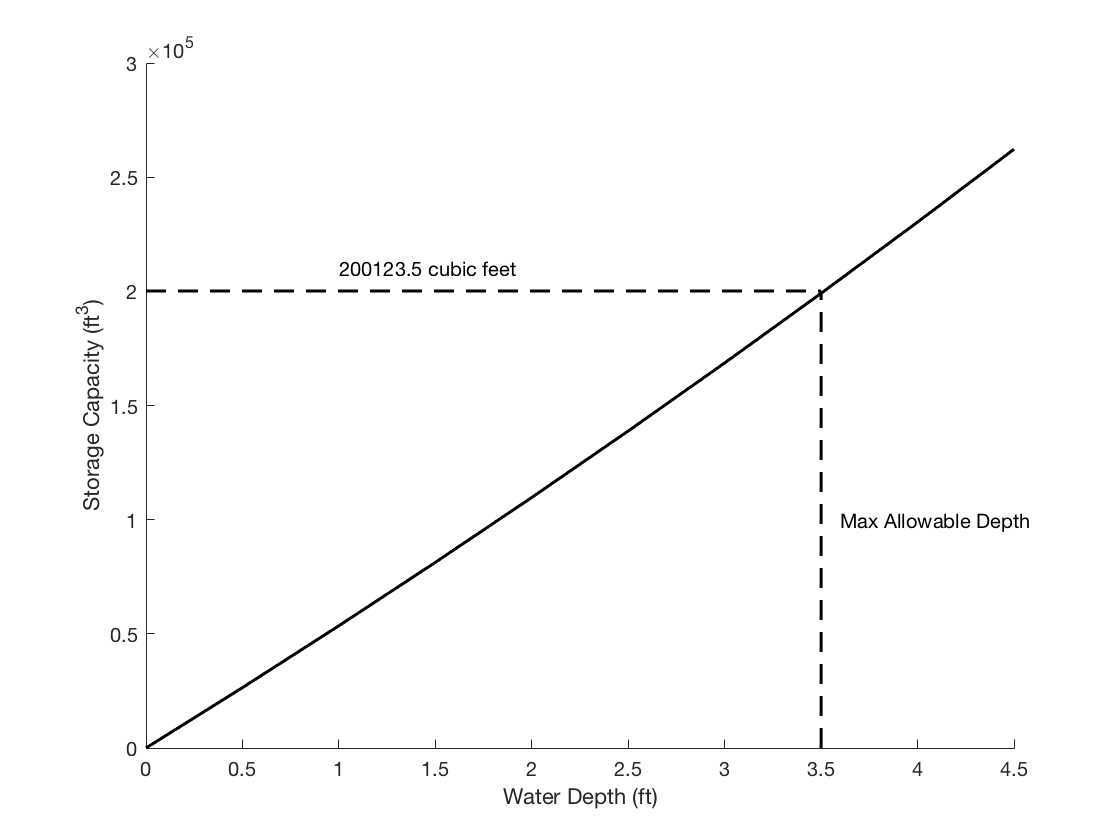
\includegraphics[height=.4\textheight]{RCP.png}

    \caption{Rating curve showing the storage volume as a function of water depth.}
\end{figure}



\section{Conclusion}

Based on the wide variety, yet striking similarity, of results, the average of all the values (except Kirpich, since it is meant for natural watersheds) displayed in Figure 1.2 is a reasonable choice (46.1 cfs). Averaging the values will minimize the effects of the variability between the results. A factor of safety will not be included in this estimate, as the freeboard included in the conveyance channel is intended to address that concern.



\setcounter{figure}{0}
\setcounter{section}{0} 
\chapter{Project Objectives}
To carry the water from the park and the concrete tarmac to the detention pond located 4,000 ft away, the conveyance channel design summarized in Table 2.1 is proposed. The required peak flow depth, velocity, and Froude number are all intended to create a channel space that is safe for all members of the community. Keeping the Froude number low keeps the energy of the flow low, keeping the velocity and the peak depth low reduces the danger of people being swept away. The freeboard is a safety factor to safeguard against abnormal behavior or more intense storms.
\begin{table}[htbp]
    \centering
    \caption{Recommended design parameters and design constraints.}
    \begin{tabular}{lcc}
    \textbf{Parameter}& \textbf{Design} & \textbf{Constraint}\\
    \hline
    Length (ft) & 4,000 &4,000   \\
    Peak Flow Depth (ft)  & 2.68 &<3.5\\
    Peak Flow Velocity (ft/s) & 1.11 & <4\\
    Peak Froude Number & 0.18 & <0.65\\
    Freeboard (ft) & 1  & 1 \\
    Peak Flow (cfs) & 46.1 & \\
    Lining & Rip-rap and vegetation &  \\
    Slope (ft/ft) & 0.0015 & \\
    Vertical Drop over 3,500 ft (ft)& 5.25 & \\
    Cross Section & Irregular &  \\
    Peak Flow Width (ft) & 35.26 & \\
    Total Initial Channel Width (ft) & 38.8\\ 
    Total Excavation Volume (yd$^3$) & 34,646 \\
    Total Footprint (acres) & 4.59 \\ \hline
    \end{tabular} 
    \end{table}

    Manning's n values for cement, grass, and brick were approximated as unfinished cement, short-grass pasture, and brick with cement mortar. The values were obtained from \cite{White} and\cite{Metcalf}, respectively.

    \begin{figure}[H]
        \centering
        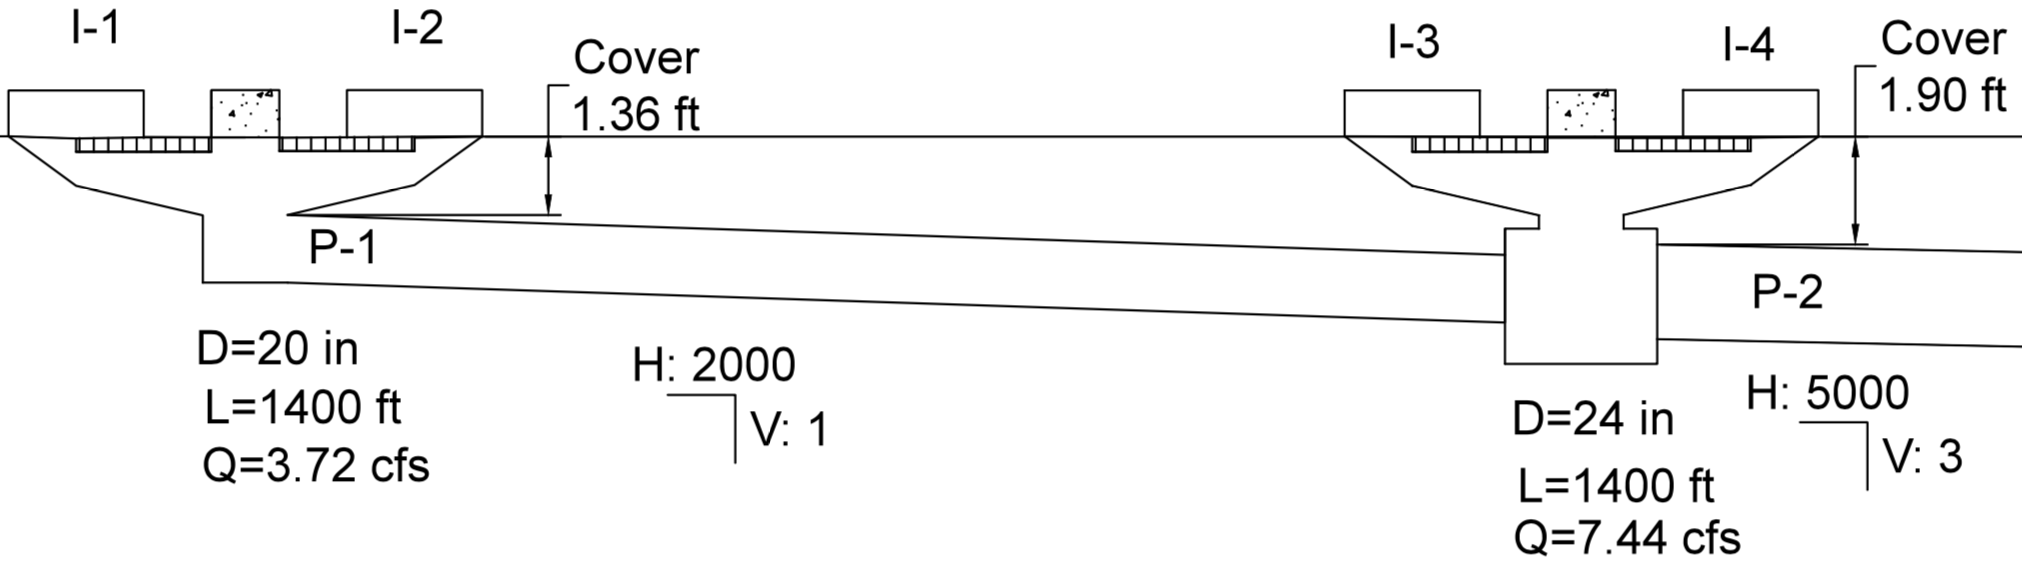
\includegraphics[width=\textwidth]{F1ss2}
        \caption{Schematic of the inlets and the storm sewer pipes. Not to Scale.}
    \end{figure}



\setcounter{figure}{0}
\setcounter{section}{0}
\setcounter{table}{0}
\chapter{Technical Approach}

To convey the water collected in the gutters and inlets mentioned previously, this section details the design of a storm sewer network. Table 4.1 contains a summary of the design parameters and Appendix D contains the technical drawings.


\begin{table}[H]
\begin{small}
\centering
\caption{Summary of design parameters. $y_n$ is the normal depth at peak flow, and D is the diameter.}
\begin{tabular}{cccccccp{15mm}c}

\textbf{Pipe}&\textbf{Material}&\textbf{Q (cfs)}&\textbf{Velocity (ft/s)}&\textbf{Diameter (in)}&\textbf{Length (ft)} & \textbf{Slope (\%)} &\centering \textbf{Crown Depth (ft)}&$\mathbf{y_n/D}$\\ \hline
P-1& PVC& 3.72 & 2.1& 20 & 1400 & 0.05 & \centering 1.36 & 0.76 \\ 
P-2& PVC &  7.44& 2.6& 24& 1400& 0.06& \centering 1.90& 0.85\\
P-3& PVC& 14.88& 3.25& 30& 100& 0.07& \centering 1.90& 0.88\\ \hline
\end{tabular}
\end{small}
\end{table}


\section{Summary}

This culvert design provides a low-cost alternatives to a bridge, as it is highly effective at both providing a crossing and conveying water. The culvert design consists of two 40 ft long, 30 in circular concrete pipes with 45$\deg$ bevels to increase inlet hydraulic efficiency. The pipes are placed at the bottom of the low flow channel to prevent the accumulation of trash and the reproduction of mosquitos. The flow velocities in the pipes were kept between 2-10 ft/s to prevent excessive scour and to prevent people or animals from being pulled in. If the soil is deemed to be suitable, the excavation material near the culvert should be used to construct the culvert to reduct construction costs. Additionally, a standard culvert pipe size and material were used to lower the cost of construction. \\~\\



\setcounter{figure}{0}
\setcounter{section}{0}
\setcounter{equation}{0}
\setcounter{table}{0}
\chapter{Deliverables}
Runoff flow rates typically increase when a watershed is developed; the grass and soil become covered in tarmac, pavement, and houses, so less water is absorbed into the soil. To prevent downstream natural ecosystems from being overwhelmed by the increased runoff, detention ponds are designed to contain the upstream channel's discharge and to release the same flowrate into the natural ecosystem as was released pre-development. Table 6.2 summarizes the detention pond and orifice design parameters. See Appendix G for additional technical drawings and for the MATLAB code used to calculate volumes.

\begin{table}[H]
    \centering
    \caption{Detention pond design parameters.}
    \begin{tabular}{lcc}
\textbf{Parameter}&\textbf{Value}&\textbf{Constraint}\\ \hline
Maximum Water Depth, 10-year Storm (ft) & 3.5 & 4 \\
Total Pond Depth (ft) & 4.5  & \\
Freeboard (ft) & 1 &  \\
Pond Storage & 200,123.5 & \\ 
Volume of Excavation (ft$^3$) & 707,233.3 & \\
Orifice Area ft$^2$& 2.85 &\\
Orifice Diameter ft & 2 & \\ \hline

\end{tabular} 
\end{table}


\section{Summary}
This detention pond design effectively manages the pre/post-development scenario and prevents downstream ecosystems from being overwhelmed. With a pre-development peak runoff flowrate of 30 cfs and the post-development value of 61 cfs, the required storage is 197,904 ft$^3$. The maximum water depth in the pond is 3.5 ft for 10-year storm and a freeboard of 1 ft is included. The depth of 3.5 ft is shallow enough to prevent residents from harming themselves should they fall into the pond. A circular pond with a flat bottom and an island in the middle was chosen for the design; the circular shape is pleasing to the eye, and the island provides habitat for beneficial insects and adds aesthetic value. The pond will be lined with the same native flora used throughout this design to ensure a seamless and natural-feeling transition between the channel and the pond. Additionally, the natural lining will facilitate infiltration to recharge groundwater supplies. A side slope of 3:1 (H:V) was chosen to allow for easy landscaping with native vegetation. Construction costs were reduced by extending the pond with a 3:1 slope to the same height as the top of the channel; otherwise, excavation costs would be many times larger. The orifice is located on the opposite side of the pond as the inlet and is sized appropriately to allow the pre-development peak runoff flowrate of 30 cfs to flow through it when the water depth reaches 3.5 ft. Orifice costs were reduced by using a standard size, corrugated metal pipe.

\setcounter{figure}{0}
\setcounter{section}{0}
\setcounter{table}{0}
\chapter{Project Management}


\setcounter{figure}{0}
\setcounter{section}{0}
\setcounter{table}{0}
\chapter{Risk Management}

\begin{figure}[H]
    \centering
    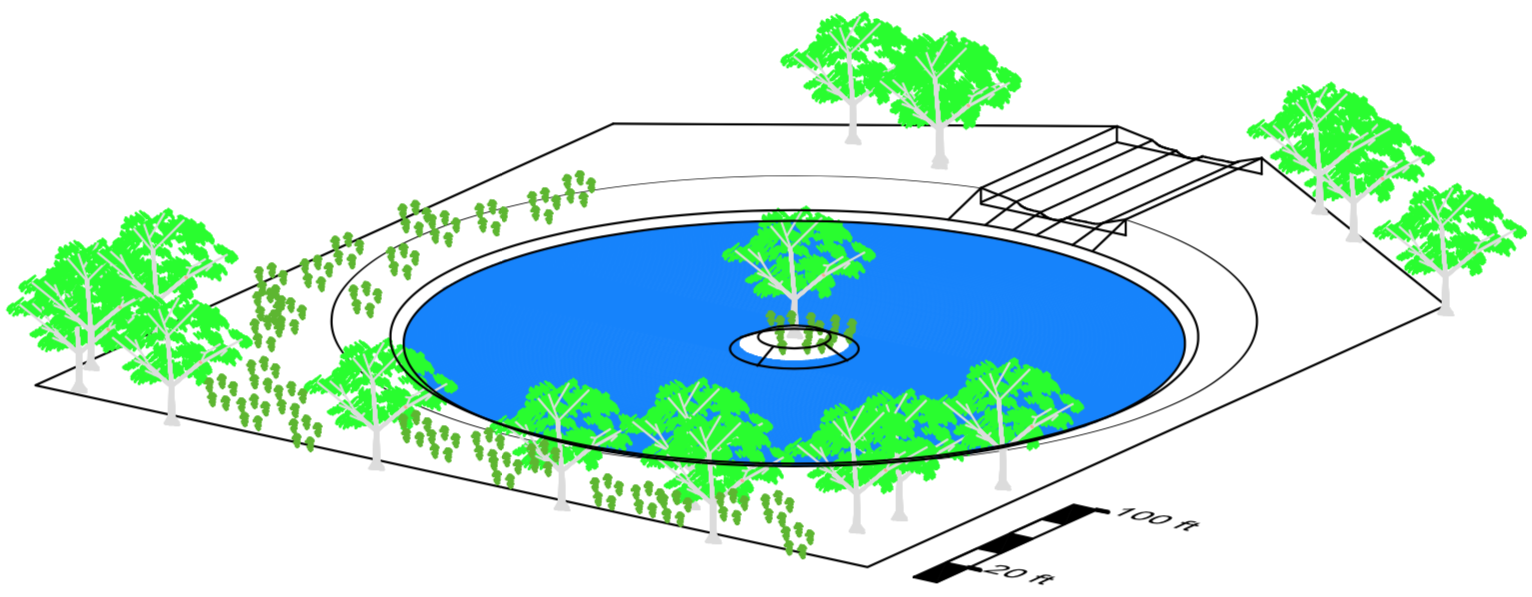
\includegraphics[height=.2\textheight]{F3P.png}
    \caption{Impression of what the pond may look like after landscaping. }
\end{figure}


\setcounter{figure}{0}
\setcounter{section}{0}
\setcounter{table}{0}
\chapter{Required Resources}

\setcounter{figure}{0}
\setcounter{section}{0}
\setcounter{table}{0}
\chapter{References}

\setcounter{figure}{0}
\setcounter{section}{0}
\setcounter{table}{0}
\chapter{Appendix A - Resumes}


\renewcommand{\thefigure}{A.\arabic{figure}}
\setcounter{figure}{0}


\begin{flushleft}
\newpage
\bibliography{bib} 
\bibliographystyle{ieeetr} 
\end{flushleft}

\end{document}
